\chapter{Propuesta}\label{chapter:proposal}

\section{Metodología}\label{sec:method}
%-----------------------------------------------------------------------------------
En este capítulo se propone una método para la detección de cáncer de piel mediante el aprendizaje automático. Este enfoque de solución se basa en la implementación de una  red neuronal profunda para analizar y categorizar automáticamente imágenes, con el objetivo de asistir en la detección de posibles casos malignos y mejorar la eficiencia del proceso diagnóstico.

A continuación, se introducen algunos de los conceptos básicos de los métodos o técnicas que se emplearan a lo largo del capítulo.
\section{Dataset}

El dataset utilizado como medio de aprendizaje para este proyecto es el Dataset: HAM1000-segmentation-and-classification  \brackcite{ham10000}. 
Este conjunto de datos, acrónimo de Human Against Machine (Humano contra máquina) con 10000 imágenes de entrenamiento, es una amplia colección de imágenes dermatoscópicas. En concreto, contiene 10015 imágenes del archivo ISIC, que inicialmente formaban parte de un conjunto de entrenamiento creado por ISIC \brackcite{tschandl2018ham10000} con la siguiente distribución.\\

\begin{tabular}{lrr}
   \hline
   \textbf{Categoría Diagnóstica} & \textbf{Número de Imágenes} & \textbf{Porcentaje} \\
   \hline
   Melanocytic nevi               & 6705                        & 66.95\%             \\
   Melanoma                       & 1113                        & 11.11\%             \\
   Benign keratosis-like lesions  & 1099                        & 10.97\%             \\
   Basal cell carcinoma           & 514                         & 5.13\%              \\
   Actinic keratoses              & 327                         & 3.27\%              \\
   Vascular lesions               & 142                         & 1.42\%              \\
   Dermatofibroma                 & 115                         & 1.15\%              \\
   \hline
   \end{tabular}

\section{Preparación y carga de datos}

Los datos utilizados como medio de aprendizaje para este proyecto son: Imágenes y Metadatos. Los datos son extraídos del Dataset: HAM1000-segmentation-and-classification  \brackcite{ham10000}.
El mismo contiene imágenes tomadas de varios tipos de cáncer de piel y contiene además un archivo Excel formato csv de Metadatos. Los metadatos contienen información relacionada con cada imagen con un formato de \textit{one hot encoding}.

\subsection{Transformación de datos}

Para optimizar la eficiencia del algoritmo, se procesan las imágenes realizando diversas modificaciones, que incluyen: eliminación de cabello, luces y sombras, división de canales y aplicación de un leve desenfoque.

Los metadatos, asociados a la clasificación, están etiquetados utilizando el método de \textit{one hot encoding}. Fue necesario convertirlos a un formato \textit{categórico} para su procesamiento.

El \textit{one hot encoding} es una técnica de procesamiento de datos en la cual cada valor categórico se representa mediante un vector binario cuyo tamaño corresponde al número de categorías posibles. En dicho vector, todos los elementos son cero, salvo el correspondiente a la categoría del valor, que es uno \brackcite{ohe}. 

Se define \textit{categórico} como el formato en el que a cada elemento se le asigna el nombre de una categoría como propiedad.

\subsection{Modelación y división del conjunto de datos}

Los datos se modelan a partir de un Dataframe de Pandas  \brackcite{pandas}. Los mismo son divididos luego en 3 conjuntos: Entrenamiento, Validación y Prueba utilizando un enfoque simple de division de datos en porcentaje. Estas divisiones son necesarias para que el modelo pueda aprender y ser evaluado correctamente. Aquí, se define que

\begin{enumerate}
   \item El 95\% de los datos se destinan al conjunto de entrenamiento.
   \item El 2.5\% de los datos restantes se destinan al conjunto de validación.
   \item El 2.5\% restante se destina al conjunto de pruebas.
\end{enumerate}
 
Además se mezclan aleatoriamente los datos y se utiliza una variable fija para garantizar que la división sea reproducible.

\begin{table}[h]
   \centering
   \begin{tabular}{lccc}
   \hline
   Diagnostic category & Training & Validation & Testing \\ \hline
   AKIEC & 122 & 4 & 1 \\
   BCC & 487 & 12 & 15 \\
   BKL & 1045 & 31 & 23 \\
   DF & 108 & 5 & 2 \\
   MEL & 1036 & 38 & 39 \\
   NV & 6389 & 154 & 162 \\
   VASC & 137 & 1 & 4 \\ \hline
   \end{tabular}
   \caption{Distribución de imágenes de cáncer de piel en Entrenamiento, Test, y Validación Datasets}
   \label{tab:train_test_validate}
   \end{table}

\section{Generadores de datos y preprocesamiento}

Uno de los principales problemas del Dataset, es el desequilibrio en la representación de las clases, un problema habitual en los conjuntos de datos médicos en los que algunas enfermedades son más raras que otras. Para solucionar este problema, el conjunto de datos se equilibra meticulosamente limitando el número máximo de muestras por clase. Esto garantiza que el modelo no esté sesgado hacia las clases más comunes y pueda generalizar mejor entre varios tipos de lesiones cutáneas.

Se detectó que el conjunto de datos estaba altamente desequilibrado. Por lo tanto, limitamos el número máximo de muestras por clase a 300 para equilibrar el conjunto de datos. Los datos con menor cantidad de muestras es debido a la disponibilidad limitada de datos originales. \\ 

\begin{table}[h]
   \centering
   \begin{tabular}{lccc}
   \hline
   Diagnostic category & Sampling  \\ \hline
   AKIEC & 300 \\
   BCC & 300 \\
   BKL & 300 \\
   DF & 115 \\
   MEL & 300 \\
   NV & 300 \\
   VASC & 142 \\ \hline
   \end{tabular}
   \caption{Distribución de muestras por categoría después del sobre-muestreo}
   \label{tab:sampling_distribution}
   \end{table}

Como se muestra anteriormente, al separar la data en clases todavía el conjunto queda desbalanceado por lo que se hace necesario aplicar otro método llamado \textit{Class Weighting} \brackcite{analyticsvidhya2020classweight}. Este método se refiere a la asignación de pesos diferenciados a cada clase durante el proceso de entrenamiento del modelo debido conjuntos de datos desequilibrados, con el objetivo de reforzar la señal de entrenamiento de las clases menos representadas, o sea, las clases/categorías con menos cantidad de datos:

\begin{table}[h]
   \centering
   \begin{tabular}{lccc}
   \hline
   Diagnostic category & Sampling  & Weighting\\ \hline
   AKIEC & 300 & 1.00\\
   BCC & 300 & 1.00\\
   BKL & 300 & 1.00\\
   DF & 115 & 2.60\\
   MEL & 300 & 1.00\\
   NV & 300 & 1.00\\
   VASC & 142 & 2.11\\ \hline
   \end{tabular}
   \caption{Distribución de Muestras con peso asignado}
   \label{tab:weighting_distribution}
   \end{table}

\subsection{Aumento y división de datos}

Para la carga y procesamiento de imágenes se utilizó la clase ImageDataGenerator de Keras \brackcite{img_gen}. Esta clase es una parte integral de la biblioteca Keras y proporciona una forma eficiente de manipular imágenes para tareas de aprendizaje automático. Su principal función es facilitar la creación de lotes de imágenes que se utilizan durante el entrenamiento y la evaluación de modelos de Machine Learning, especialmente en el contexto de redes neuronales. 

Se inicializa con varias transformaciones (como rotación, desplazamiento y zoom) para aplicar automáticamente estas transformaciones a las imágenes a medida que se cargan devolver lotes de imágenes listos para el entrenamiento o la evaluación del modelo, lo cual permite alimentar la red neuronal de manera eficiente \brackcite{augmentation}.

\begin{table}[h]
   \centering
   \begin{tabular}{lccc}
   \hline
   Parámetro & Descripción  & Valor \\ \hline
   rotation range & 	Rango de rotación & 20 grados \\
   width shift range & Rango de desplazamiento horizontal & 20\% \\
   height shift range & Rango de desplazamiento vertical & 20\% \\
   shear range & 	Rango de corte & 20\% \\
   zoom range & Rango de zoom & 20\% \\
   horizontal flip & Activación de volteo horizontal & verdadero \\
   fill mode & Modo de relleno para manejar los píxeles faltantes & nearest \\ \hline
   \end{tabular}
   \caption{Parámetros de aumento de datos}
   \label{tab:data_augmentation_params}
   \end{table}

\section{Diseño y entrenamiento del modelo}

Se utiliza la arquitectura de red neural denominada \textit{EfficientNetB5} \brackcite{efficientnet}. Esta arquitectura forma parte de la familia EfficientNet, que está diseñada para proporcionar alta precisión mientras se mantiene un tamaño de modelo y una complejidad computacional eficientes.

Para aprovechar los conocimientos previos y acelerar el entrenamiento, se carga el modelo \textit{EfficientNetB5} pre-entrenado con los pesos obtenidos de entrenar en el dataset \textit{ImageNet}, que es una amplia base de datos de imágenes utilizada comúnmente para entrenamiento y \textit{benchmarking} en tareas de visión por computadora. Utilizar un modelo pre-entrenado permite aprovechar las características que ya ha aprendido de este amplio conjunto de datos, facilitando su adaptación al dataset.

Se utiliza el \textit{EfficientNetB5} sin incluir su capa superior, con el objetivo de añadir y personalizar capas adicionales. Tras obtener la salida del modelo base, se aplica una serie de transformaciones, incluyendo normalización por lotes, una capa densa con regularizaciones, una técnica de \textit{Dropout} para prevenir el sobre-ajuste y una capa de optimización. 

\subsection{ImageNet}

ImageNet es un proyecto de base de datos visual extenso, diseñado principalmente para la investigación en reconocimiento visual de objetos. Contiene más de 14 millones de imágenes, anotadas manualmente para indicar qué objetos se muestran, y más de 20,000 categorías, cada una con cientos o miles de imágenes. Este proyecto ha sido fundamental en el avance de la visión por computadora y el aprendizaje profundo, proporcionando un recurso de datos inmenso y diverso para entrenar algoritmos de inteligencia artificial.

La relevancia de ImageNet para el aprendizaje profundo se puso de manifiesto con el éxito de AlexNet en el desafío ImageNet 2012 \brackcite{Pinecone2021ImageNet}, donde logró una tasa de error top-5 del 15.3\%, notablemente inferior a la de sus competidores. Este hito marcó un punto de inflexión en el campo, demostrando la viabilidad y la potencia de las redes neuronales convolucionales (CNN) cuando se combinan con unidades de procesamiento gráfico (GPU) para el entrenamiento.

\subsection{Arquitectura del modelo EfficientNet}

La familia de arquitecturas EfficientNet, desarrollada por los autores en \brackcite{tan2019efficientnet}, surgió con el objetivo de hallar un método adecuado para escalar las CNNs de manera que mejoraran tanto en precisión (es decir, rendimiento del modelo) como en eficiencia (es decir, en términos de parámetros del modelo y FLOPS). Estos autores propusieron un método de escalado compuesto que utiliza un conjunto fijo de coeficientes para escalar de manera uniforme el ancho, la profundidad y la resolución de la red. Este método les permitió desarrollar una arquitectura de CNN eficiente, a la que denominaron EfficientNet B0. Posteriormente, crearon las variantes EfficientNets B1-B7 escalando la red base (EfficientNet B0).

Mientras que la arquitectura EfficientNet B0 tiene 5.3 millones de parámetros y acepta imágenes de entrada de 224x224, EfficientNet B7 cuenta con 66 millones de parámetros y acepta imágenes de 600x600. \brackcite{Tan2019EfficientNetRM}

\begin{figure}[ht]%
   \begin{center}
   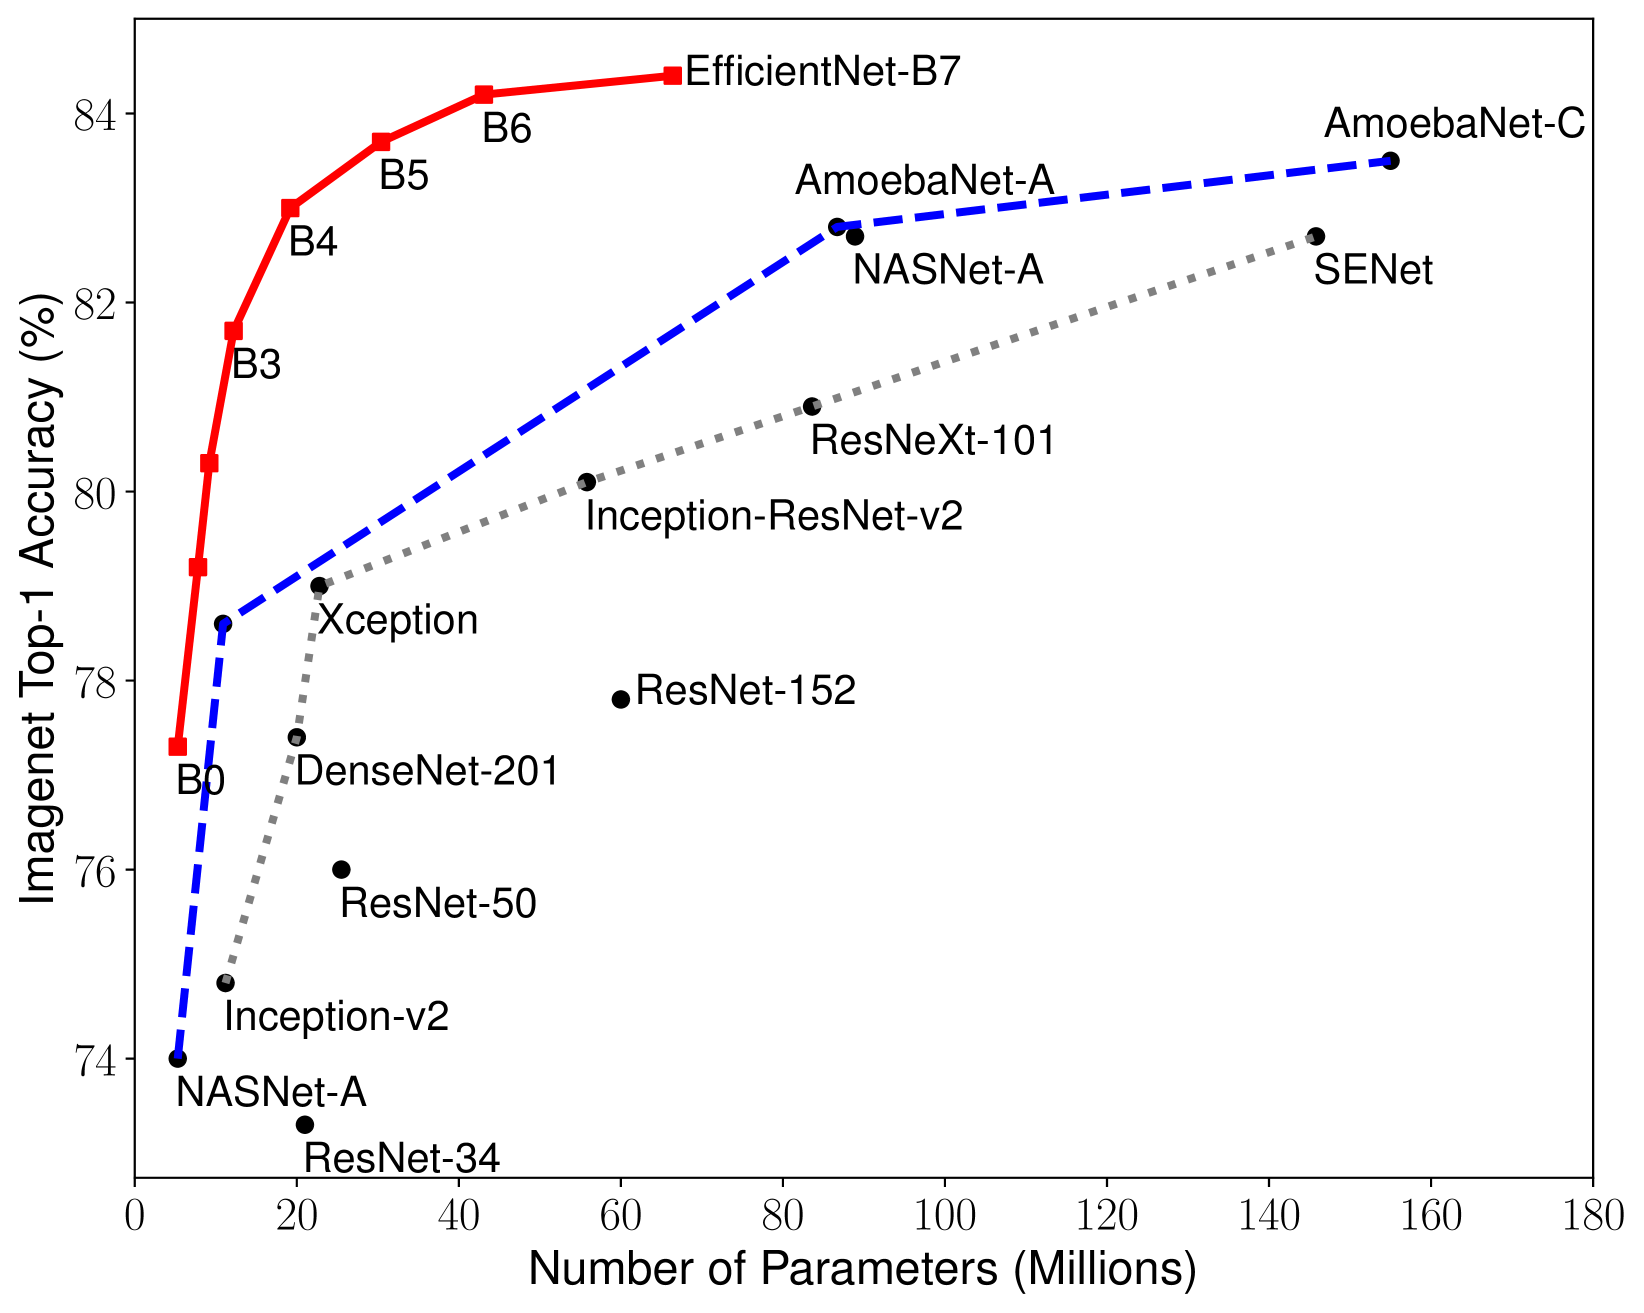
\includegraphics[width=0.45\textwidth]{./Graphics/efficientnet_performance.png}
   \caption{Estadísticas del rendimiento de los modelos de EfficientNet}
   \label{fig:efficientnet_performance}
   \end{center}
   \end{figure}

\subsection{EfficientNetB5}

En relación con el Dataset HAM1000 \brackcite{ham10000}, la implementación del EfficientNetB5 puede ser particularmente beneficiosa para el análisis de datos. EfficientNetB5 es una de las variantes de la serie EfficientNet, que se encuentra en un punto medio en términos de complejidad y tamaño, ofreciendo un equilibrio entre precisión y eficiencia computacional. Dado que el HAM1000 es un conjunto de datos de imágenes dermatoscópicas que requiere una alta precisión en la identificación y clasificación de lesiones cutáneas, la utilización de EfficientNetB5 podría proporcionar una precisión y eficiencia aceptable en términos de recursos computacionales.

EfficientNetB5, con su capacidad para manejar imágenes de mayor resolución y su arquitectura optimizada, se considero para este trabajo más adecuado para captar las características detalladas y sutilezas en las imágenes dermatológicas. Esta capacidad es crucial para distinguir entre diferentes tipos de lesiones cutáneas, lo que a menudo requiere un análisis detallado de texturas, colores y patrones. Además, el uso de un modelo pre-entrenado en ImageNet proporciona una base sólida de características generales, que puede ser más afinada y adaptada a las especificidades del dataset HAM1000.

\subsection{Capas adicionales y regularización}

Para ajustar el modelo de EfficientNetB5 a nuestras necesidades, se añaden capas adicionales:

\begin{enumerate}
   \item Normalización por lotes: Esta capa busca estandarizar las activaciones del modelo para cada lote de entrenamiento. 
   La misma regulariza el modelo y, al mismo tiempo, suele acelera el entrenamiento ya que permite utilizar tasas de aprendizaje más altas. [\brackcite{regularization}]

   \item Densa: Se introduce una capa completamente conectada con 256 neuronas. Esta capa tiene una activación ReLU y utiliza regularización L1 y L2.
   La regularización L1 y L2 penaliza los pesos grandes en la red, ayudando a evitar el sobre-ajuste y garantizando que el modelo se generalice
    bien a nuevos datos. \brackcite{dense}
   
   \item Dropout: Esta técnica de regularización desactiva aleatoriamente una fracción (en este caso, el 45\%) de las neuronas durante el 
   entrenamiento. Esta aleatoriedad ayuda a evitar la dependencia excesiva en cualquier neurona individual, lo que a su vez ayuda a prevenir
    el sobre-ajuste. \brackcite{dropout}
   
   \item Capa de salida: Finalmente, se agrega una capa densa que tiene un número de neuronas igual al número de clases en nuestro problema. 
   La activación \textit{softmax} se utiliza aquí para transformar las salidas en probabilidades de clase.

\end{enumerate}

\subsection{Optimización}

Para el proceso de entrenamiento, se utiliza el optimizador \textit{Adamax} \brackcite{adamax}. Este es una variante del conocido optimizador Adam, que combina las ventajas de los métodos adaptativos de tasa de aprendizaje con una implementación más robusta en presencia de momentos espurios. 

Se configura el modelo para minimizar la categorical crossentropy, que es una medida común de error para problemas de clasificación, y se rastrea la precisión como métrica principal.

\subsection{Ajusted dinámico de la tasa de aprendizaje}

Una de las características más innovadoras de este enfoque es la inclusión de un "Callback" personalizado para ajustar dinámicamente la tasa de aprendizaje durante el entrenamiento. Este ajuste se basa en la precisión del entrenamiento y la pérdida de validación. En resumen, si el modelo no mejora lo suficientemente rápido (según ciertos criterios preestablecidos), la tasa de aprendizaje se reduce, con la esperanza de mejorar la convergencia del modelo \brackcite{lr}.

Este enfoque puede ser especialmente útil cuando nos enfrentamos a superficies de pérdida complejas con múltiples mínimos locales; al variar la tasa de aprendizaje, es más probable que el modelo salga de mínimos locales subóptimos y encuentre una solución mejor.
